\documentclass[1p]{elsarticle_modified}
%\bibliographystyle{elsarticle-num}

%\usepackage[colorlinks]{hyperref}
%\usepackage{abbrmath_seonhwa} %\Abb, \Ascr, \Acal ,\Abf, \Afrak
\usepackage{amsfonts}
\usepackage{amssymb}
\usepackage{amsmath}
\usepackage{amsthm}
\usepackage{scalefnt}
\usepackage{amsbsy}
\usepackage{kotex}
\usepackage{caption}
\usepackage{subfig}
\usepackage{color}
\usepackage{graphicx}
\usepackage{xcolor} %% white, black, red, green, blue, cyan, magenta, yellow
\usepackage{float}
\usepackage{setspace}
\usepackage{hyperref}

\usepackage{tikz}
\usetikzlibrary{arrows}

\usepackage{multirow}
\usepackage{array} % fixed length table
\usepackage{hhline}

%%%%%%%%%%%%%%%%%%%%%
\makeatletter
\renewcommand*\env@matrix[1][\arraystretch]{%
	\edef\arraystretch{#1}%
	\hskip -\arraycolsep
	\let\@ifnextchar\new@ifnextchar
	\array{*\c@MaxMatrixCols c}}
\makeatother %https://tex.stackexchange.com/questions/14071/how-can-i-increase-the-line-spacing-in-a-matrix
%%%%%%%%%%%%%%%

\usepackage[normalem]{ulem}

\newcommand{\msout}[1]{\ifmmode\text{\sout{\ensuremath{#1}}}\else\sout{#1}\fi}
%SOURCE: \msout is \stkout macro in https://tex.stackexchange.com/questions/20609/strikeout-in-math-mode

\newcommand{\cancel}[1]{
	\ifmmode
	{\color{red}\msout{#1}}
	\else
	{\color{red}\sout{#1}}
	\fi
}

\newcommand{\add}[1]{
	{\color{blue}\uwave{#1}}
}

\newcommand{\replace}[2]{
	\ifmmode
	{\color{red}\msout{#1}}{\color{blue}\uwave{#2}}
	\else
	{\color{red}\sout{#1}}{\color{blue}\uwave{#2}}
	\fi
}

\newcommand{\Sol}{\mathcal{S}} %segment
\newcommand{\D}{D} %diagram
\newcommand{\A}{\mathcal{A}} %arc


%%%%%%%%%%%%%%%%%%%%%%%%%%%%%5 test

\def\sl{\operatorname{\textup{SL}}(2,\Cbb)}
\def\psl{\operatorname{\textup{PSL}}(2,\Cbb)}
\def\quan{\mkern 1mu \triangleright \mkern 1mu}

\theoremstyle{definition}
\newtheorem{thm}{Theorem}[section]
\newtheorem{prop}[thm]{Proposition}
\newtheorem{lem}[thm]{Lemma}
\newtheorem{ques}[thm]{Question}
\newtheorem{cor}[thm]{Corollary}
\newtheorem{defn}[thm]{Definition}
\newtheorem{exam}[thm]{Example}
\newtheorem{rmk}[thm]{Remark}
\newtheorem{alg}[thm]{Algorithm}

\newcommand{\I}{\sqrt{-1}}
\begin{document}

%\begin{frontmatter}
%
%\title{Boundary parabolic representations of knots up to 8 crossings}
%
%%% Group authors per affiliation:
%\author{Yunhi Cho} 
%\address{Department of Mathematics, University of Seoul, Seoul, Korea}
%\ead{yhcho@uos.ac.kr}
%
%
%\author{Seonhwa Kim} %\fnref{s_kim}}
%\address{Center for Geometry and Physics, Institute for Basic Science, Pohang, 37673, Korea}
%\ead{ryeona17@ibs.re.kr}
%
%\author{Hyuk Kim}
%\address{Department of Mathematical Sciences, Seoul National University, Seoul 08826, Korea}
%\ead{hyukkim@snu.ac.kr}
%
%\author{Seokbeom Yoon}
%\address{Department of Mathematical Sciences, Seoul National University, Seoul, 08826,  Korea}
%\ead{sbyoon15@snu.ac.kr}
%
%\begin{abstract}
%We find all boundary parabolic representation of knots up to 8 crossings.
%
%\end{abstract}
%\begin{keyword}
%    \MSC[2010] 57M25 
%\end{keyword}
%
%\end{frontmatter}

%\linenumbers
%\tableofcontents
%
\newcommand\colored[1]{\textcolor{white}{\rule[-0.35ex]{0.8em}{1.4ex}}\kern-0.8em\color{red} #1}%
%\newcommand\colored[1]{\textcolor{white}{ #1}\kern-2.17ex	\textcolor{white}{ #1}\kern-1.81ex	\textcolor{white}{ #1}\kern-2.15ex\color{red}#1	}

{\Large $\underline{11a_{30}~(K11a_{30})}$}

\setlength{\tabcolsep}{10pt}
\renewcommand{\arraystretch}{1.6}
\vspace{1cm}\begin{tabular}{m{100pt}>{\centering\arraybackslash}m{274pt}}
\multirow{5}{120pt}{
	\centering
	\includegraphics[width=112pt]{../../../GIT/diagram.site/Diagrams/png/279_11a_30.png}\\
\ \ \ A knot diagram\footnotemark}&
\allowdisplaybreaks
\textbf{Linearized knot diagam} \\
\cline{2-2}
 &
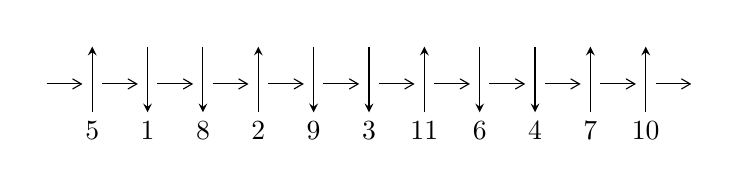
\begin{tikzpicture}[x=20pt, y=17pt]
	% nodes
	\node (C0) at (0, 0) {};
	\node (C1) at (1, 0) {};
	\node (C1U) at (1, +1) {};
	\node (C1D) at (1, -1) {5};

	\node (C2) at (2, 0) {};
	\node (C2U) at (2, +1) {};
	\node (C2D) at (2, -1) {1};

	\node (C3) at (3, 0) {};
	\node (C3U) at (3, +1) {};
	\node (C3D) at (3, -1) {8};

	\node (C4) at (4, 0) {};
	\node (C4U) at (4, +1) {};
	\node (C4D) at (4, -1) {2};

	\node (C5) at (5, 0) {};
	\node (C5U) at (5, +1) {};
	\node (C5D) at (5, -1) {9};

	\node (C6) at (6, 0) {};
	\node (C6U) at (6, +1) {};
	\node (C6D) at (6, -1) {3};

	\node (C7) at (7, 0) {};
	\node (C7U) at (7, +1) {};
	\node (C7D) at (7, -1) {11};

	\node (C8) at (8, 0) {};
	\node (C8U) at (8, +1) {};
	\node (C8D) at (8, -1) {6};

	\node (C9) at (9, 0) {};
	\node (C9U) at (9, +1) {};
	\node (C9D) at (9, -1) {4};

	\node (C10) at (10, 0) {};
	\node (C10U) at (10, +1) {};
	\node (C10D) at (10, -1) {7};

	\node (C11) at (11, 0) {};
	\node (C11U) at (11, +1) {};
	\node (C11D) at (11, -1) {10};
	\node (C12) at (12, 0) {};

	% arrows
	\draw[->,>={angle 60}]
	(C0) edge (C1) (C1) edge (C2) (C2) edge (C3) (C3) edge (C4) (C4) edge (C5) (C5) edge (C6) (C6) edge (C7) (C7) edge (C8) (C8) edge (C9) (C9) edge (C10) (C10) edge (C11) (C11) edge (C12) ;	\draw[->,>=stealth]
	(C1D) edge (C1U) (C2U) edge (C2D) (C3U) edge (C3D) (C4D) edge (C4U) (C5U) edge (C5D) (C6U) edge (C6D) (C7D) edge (C7U) (C8U) edge (C8D) (C9U) edge (C9D) (C10D) edge (C10U) (C11D) edge (C11U) ;
	\end{tikzpicture} \\
\hhline{~~} \\& 
\textbf{Solving Sequence} \\ \cline{2-2} 
 &
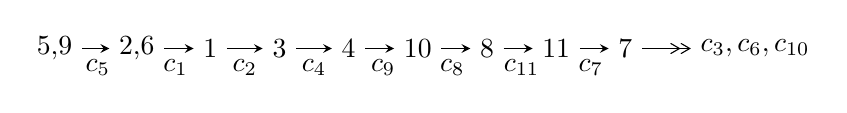
\begin{tikzpicture}[x=25pt, y=7pt]
	% node
	\node (A0) at (-1/8, 0) {5,9};
	\node (A1) at (17/16, 0) {2,6};
	\node (A2) at (17/8, 0) {1};
	\node (A3) at (25/8, 0) {3};
	\node (A4) at (33/8, 0) {4};
	\node (A5) at (41/8, 0) {10};
	\node (A6) at (49/8, 0) {8};
	\node (A7) at (57/8, 0) {11};
	\node (A8) at (65/8, 0) {7};
	\node (C1) at (1/2, -1) {$c_{5}$};
	\node (C2) at (13/8, -1) {$c_{1}$};
	\node (C3) at (21/8, -1) {$c_{2}$};
	\node (C4) at (29/8, -1) {$c_{4}$};
	\node (C5) at (37/8, -1) {$c_{9}$};
	\node (C6) at (45/8, -1) {$c_{8}$};
	\node (C7) at (53/8, -1) {$c_{11}$};
	\node (C8) at (61/8, -1) {$c_{7}$};
	\node (A9) at (10, 0) {$c_{3},c_{6},c_{10}$};

	% edge
	\draw[->,>=stealth]	
	(A0) edge (A1) (A1) edge (A2) (A2) edge (A3) (A3) edge (A4) (A4) edge (A5) (A5) edge (A6) (A6) edge (A7) (A7) edge (A8) ;
	\draw[->>,>={angle 60}]	
	(A8) edge (A9);
\end{tikzpicture} \\ 

\end{tabular} \\

\footnotetext{
The image of knot diagram is generated by the software ``\textbf{Draw programme}" developed by Andrew Bartholomew(\url{http://www.layer8.co.uk/maths/draw/index.htm\#Running-draw}), where we modified some parts for our purpose(\url{https://github.com/CATsTAILs/LinksPainter}).
}\phantom \\ \newline 
\centering \textbf{Ideals for irreducible components\footnotemark of $X_{\text{par}}$} 
 
\begin{align*}
I^u_{1}&=\langle 
7.58522\times10^{150} u^{73}+3.69824\times10^{151} u^{72}+\cdots+2.11703\times10^{151} b-1.30679\times10^{151},\\
\phantom{I^u_{1}}&\phantom{= \langle  }1.34088\times10^{151} u^{73}+4.14720\times10^{151} u^{72}+\cdots+2.11703\times10^{151} a-7.19346\times10^{151},\;u^{74}+5 u^{73}+\cdots+3 u+1\rangle \\
\\
\end{align*}
\raggedright * 1 irreducible components of $\dim_{\mathbb{C}}=0$, with total 74 representations.\\
\footnotetext{All coefficients of polynomials are rational numbers. But the coefficients are sometimes approximated in decimal forms when there is not enough margin.}
\newpage
\renewcommand{\arraystretch}{1}
\centering \section*{I. $I^u_{1}= \langle 7.59\times10^{150} u^{73}+3.70\times10^{151} u^{72}+\cdots+2.12\times10^{151} b-1.31\times10^{151},\;1.34\times10^{151} u^{73}+4.15\times10^{151} u^{72}+\cdots+2.12\times10^{151} a-7.19\times10^{151},\;u^{74}+5 u^{73}+\cdots+3 u+1 \rangle$}
\flushleft \textbf{(i) Arc colorings}\\
\begin{tabular}{m{7pt} m{180pt} m{7pt} m{180pt} }
\flushright $a_{5}=$&$\begin{pmatrix}1\\0\end{pmatrix}$ \\
\flushright $a_{9}=$&$\begin{pmatrix}0\\u\end{pmatrix}$ \\
\flushright $a_{2}=$&$\begin{pmatrix}-0.633380 u^{73}-1.95897 u^{72}+\cdots-1.62167 u+3.39790\\-0.358296 u^{73}-1.74690 u^{72}+\cdots-2.41832 u+0.617277\end{pmatrix}$ \\
\flushright $a_{6}=$&$\begin{pmatrix}1\\u^2\end{pmatrix}$ \\
\flushright $a_{1}=$&$\begin{pmatrix}-0.275084 u^{73}-0.212070 u^{72}+\cdots+0.796648 u+2.78063\\-0.358296 u^{73}-1.74690 u^{72}+\cdots-2.41832 u+0.617277\end{pmatrix}$ \\
\flushright $a_{3}=$&$\begin{pmatrix}-1.99536 u^{73}-8.76954 u^{72}+\cdots-4.79281 u+2.43887\\-0.179627 u^{73}-0.746401 u^{72}+\cdots-1.87519 u+0.121634\end{pmatrix}$ \\
\flushright $a_{4}=$&$\begin{pmatrix}-2.11453 u^{73}-9.34193 u^{72}+\cdots-5.30085 u+1.98157\\-0.294975 u^{73}-1.37123 u^{72}+\cdots-2.33439 u-0.359107\end{pmatrix}$ \\
\flushright $a_{10}=$&$\begin{pmatrix}-10.0014 u^{73}-53.9101 u^{72}+\cdots-19.0788 u-3.70357\\0.992329 u^{73}+5.03105 u^{72}+\cdots+5.38895 u+0.998316\end{pmatrix}$ \\
\flushright $a_{8}=$&$\begin{pmatrix}u\\u^3+u\end{pmatrix}$ \\
\flushright $a_{11}=$&$\begin{pmatrix}7.15691 u^{73}+29.9861 u^{72}+\cdots-18.6635 u-6.17364\\-1.14246 u^{73}-5.02812 u^{72}+\cdots-5.85728 u+0.414142\end{pmatrix}$ \\
\flushright $a_{7}=$&$\begin{pmatrix}-2.25610 u^{73}-2.17362 u^{72}+\cdots+32.2123 u+10.8684\\0.846917 u^{73}+3.12950 u^{72}+\cdots+2.74742 u-0.602325\end{pmatrix}$\\ \flushright $a_{7}=$&$\begin{pmatrix}-2.25610 u^{73}-2.17362 u^{72}+\cdots+32.2123 u+10.8684\\0.846917 u^{73}+3.12950 u^{72}+\cdots+2.74742 u-0.602325\end{pmatrix}$\\&\end{tabular}
\flushleft \textbf{(ii) Obstruction class $= -1$}\\~\\
\flushleft \textbf{(iii) Cusp Shapes $= 1.48586 u^{73}+14.4117 u^{72}+\cdots+21.1776 u-3.60826$}\\~\\
\newpage\renewcommand{\arraystretch}{1}
\flushleft \textbf{(iv) u-Polynomials at the component}\newline \\
\begin{tabular}{m{50pt}|m{274pt}}
Crossings & \hspace{64pt}u-Polynomials at each crossing \\
\hline $$\begin{aligned}c_{1},c_{4}\end{aligned}$$&$\begin{aligned}
&u^{74}+u^{73}+\cdots+u+1
\end{aligned}$\\
\hline $$\begin{aligned}c_{2}\end{aligned}$$&$\begin{aligned}
&u^{74}+29 u^{73}+\cdots+57 u+1
\end{aligned}$\\
\hline $$\begin{aligned}c_{3}\end{aligned}$$&$\begin{aligned}
&u^{74}- u^{73}+\cdots-11 u+1
\end{aligned}$\\
\hline $$\begin{aligned}c_{5},c_{8}\end{aligned}$$&$\begin{aligned}
&u^{74}-5 u^{73}+\cdots-3 u+1
\end{aligned}$\\
\hline $$\begin{aligned}c_{6}\end{aligned}$$&$\begin{aligned}
&u^{74}-5 u^{73}+\cdots-355 u+199
\end{aligned}$\\
\hline $$\begin{aligned}c_{7},c_{10}\end{aligned}$$&$\begin{aligned}
&u^{74}-5 u^{73}+\cdots-3 u+1
\end{aligned}$\\
\hline $$\begin{aligned}c_{9}\end{aligned}$$&$\begin{aligned}
&u^{74}-15 u^{73}+\cdots+10283 u+547
\end{aligned}$\\
\hline $$\begin{aligned}c_{11}\end{aligned}$$&$\begin{aligned}
&u^{74}-31 u^{73}+\cdots+5 u+1
\end{aligned}$\\
\hline
\end{tabular}\\~\\
\newpage\renewcommand{\arraystretch}{1}
\flushleft \textbf{(v) Riley Polynomials at the component}\newline \\
\begin{tabular}{m{50pt}|m{274pt}}
Crossings & \hspace{64pt}Riley Polynomials at each crossing \\
\hline $$\begin{aligned}c_{1},c_{4}\end{aligned}$$&$\begin{aligned}
&y^{74}+29 y^{73}+\cdots+57 y+1
\end{aligned}$\\
\hline $$\begin{aligned}c_{2}\end{aligned}$$&$\begin{aligned}
&y^{74}+33 y^{73}+\cdots-859 y+1
\end{aligned}$\\
\hline $$\begin{aligned}c_{3}\end{aligned}$$&$\begin{aligned}
&y^{74}+5 y^{73}+\cdots+33 y+1
\end{aligned}$\\
\hline $$\begin{aligned}c_{5},c_{8}\end{aligned}$$&$\begin{aligned}
&y^{74}+53 y^{73}+\cdots+5 y+1
\end{aligned}$\\
\hline $$\begin{aligned}c_{6}\end{aligned}$$&$\begin{aligned}
&y^{74}-63 y^{73}+\cdots+1039717 y+39601
\end{aligned}$\\
\hline $$\begin{aligned}c_{7},c_{10}\end{aligned}$$&$\begin{aligned}
&y^{74}-31 y^{73}+\cdots+5 y+1
\end{aligned}$\\
\hline $$\begin{aligned}c_{9}\end{aligned}$$&$\begin{aligned}
&y^{74}+105 y^{73}+\cdots-37429635 y+299209
\end{aligned}$\\
\hline $$\begin{aligned}c_{11}\end{aligned}$$&$\begin{aligned}
&y^{74}+25 y^{73}+\cdots+5 y+1
\end{aligned}$\\
\hline
\end{tabular}\\~\\
\newpage\flushleft \textbf{(vi) Complex Volumes and Cusp Shapes}
$$\begin{array}{c|c|c}  
\text{Solutions to }I^u_{1}& \I (\text{vol} + \sqrt{-1}CS) & \text{Cusp shape}\\
 \hline 
\begin{aligned}
u &= \phantom{-}0.625887 + 0.806388 I \\
a &= \phantom{-}0.250075 - 1.091350 I \\
b &= -0.155697 - 0.809103 I\end{aligned}
 & -1.13641 - 1.44571 I & \phantom{-0.000000 } 0 \\ \hline\begin{aligned}
u &= \phantom{-}0.625887 - 0.806388 I \\
a &= \phantom{-}0.250075 + 1.091350 I \\
b &= -0.155697 + 0.809103 I\end{aligned}
 & -1.13641 + 1.44571 I & \phantom{-0.000000 } 0 \\ \hline\begin{aligned}
u &= -0.948725 + 0.166866 I \\
a &= -0.188753 + 0.646780 I \\
b &= -0.755320 + 0.469376 I\end{aligned}
 & \phantom{-}0.70694 + 6.29193 I & \phantom{-0.000000 } 0 \\ \hline\begin{aligned}
u &= -0.948725 - 0.166866 I \\
a &= -0.188753 - 0.646780 I \\
b &= -0.755320 - 0.469376 I\end{aligned}
 & \phantom{-}0.70694 - 6.29193 I & \phantom{-0.000000 } 0 \\ \hline\begin{aligned}
u &= -0.018872 + 1.052340 I \\
a &= \phantom{-}0.07987 + 7.64537 I \\
b &= \phantom{-}0.488379 - 0.853979 I\end{aligned}
 & \phantom{-}1.62217 + 0.05885 I & \phantom{-0.000000 } 0 \\ \hline\begin{aligned}
u &= -0.018872 - 1.052340 I \\
a &= \phantom{-}0.07987 - 7.64537 I \\
b &= \phantom{-}0.488379 + 0.853979 I\end{aligned}
 & \phantom{-}1.62217 - 0.05885 I & \phantom{-0.000000 } 0 \\ \hline\begin{aligned}
u &= -0.212838 + 1.055230 I \\
a &= -1.05204 + 1.70067 I \\
b &= \phantom{-}0.448860 + 1.081110 I\end{aligned}
 & \phantom{-}1.70570 + 3.66146 I & \phantom{-0.000000 } 0 \\ \hline\begin{aligned}
u &= -0.212838 - 1.055230 I \\
a &= -1.05204 - 1.70067 I \\
b &= \phantom{-}0.448860 - 1.081110 I\end{aligned}
 & \phantom{-}1.70570 - 3.66146 I & \phantom{-0.000000 } 0 \\ \hline\begin{aligned}
u &= -0.046860 + 0.912129 I \\
a &= \phantom{-}1.70545 + 5.91576 I \\
b &= \phantom{-}0.473139 + 0.843516 I\end{aligned}
 & \phantom{-}1.60692 + 3.97998 I & \phantom{-}10.4876 - 34.2104 I \\ \hline\begin{aligned}
u &= -0.046860 - 0.912129 I \\
a &= \phantom{-}1.70545 - 5.91576 I \\
b &= \phantom{-}0.473139 - 0.843516 I\end{aligned}
 & \phantom{-}1.60692 - 3.97998 I & \phantom{-}10.4876 + 34.2104 I\\
 \hline 
 \end{array}$$\newpage$$\begin{array}{c|c|c}  
\text{Solutions to }I^u_{1}& \I (\text{vol} + \sqrt{-1}CS) & \text{Cusp shape}\\
 \hline 
\begin{aligned}
u &= \phantom{-}0.837681 + 0.298700 I \\
a &= \phantom{-}0.88363 + 1.74577 I \\
b &= -0.196875 + 1.092950 I\end{aligned}
 & -5.52578 - 1.17971 I & -8.59982 + 0. I\phantom{ +0.000000I} \\ \hline\begin{aligned}
u &= \phantom{-}0.837681 - 0.298700 I \\
a &= \phantom{-}0.88363 - 1.74577 I \\
b &= -0.196875 - 1.092950 I\end{aligned}
 & -5.52578 + 1.17971 I & -8.59982 + 0. I\phantom{ +0.000000I} \\ \hline\begin{aligned}
u &= -1.134810 + 0.070313 I \\
a &= \phantom{-}0.13504 - 1.56031 I \\
b &= -0.625155 - 1.073360 I\end{aligned}
 & -1.05098 + 11.53100 I & \phantom{-0.000000 } 0 \\ \hline\begin{aligned}
u &= -1.134810 - 0.070313 I \\
a &= \phantom{-}0.13504 + 1.56031 I \\
b &= -0.625155 + 1.073360 I\end{aligned}
 & -1.05098 - 11.53100 I & \phantom{-0.000000 } 0 \\ \hline\begin{aligned}
u &= -0.187862 + 1.125480 I \\
a &= -1.08777 + 1.12032 I \\
b &= \phantom{-}0.613032 + 1.148640 I\end{aligned}
 & \phantom{-}1.81406 + 3.75257 I & \phantom{-0.000000 } 0 \\ \hline\begin{aligned}
u &= -0.187862 - 1.125480 I \\
a &= -1.08777 - 1.12032 I \\
b &= \phantom{-}0.613032 - 1.148640 I\end{aligned}
 & \phantom{-}1.81406 - 3.75257 I & \phantom{-0.000000 } 0 \\ \hline\begin{aligned}
u &= \phantom{-}0.100705 + 1.152450 I \\
a &= \phantom{-}0.772241 + 0.259406 I \\
b &= -0.044485 - 0.183329 I\end{aligned}
 & \phantom{-}1.47076 - 2.21494 I & \phantom{-0.000000 } 0 \\ \hline\begin{aligned}
u &= \phantom{-}0.100705 - 1.152450 I \\
a &= \phantom{-}0.772241 - 0.259406 I \\
b &= -0.044485 + 0.183329 I\end{aligned}
 & \phantom{-}1.47076 + 2.21494 I & \phantom{-0.000000 } 0 \\ \hline\begin{aligned}
u &= \phantom{-}0.818597 + 0.196251 I \\
a &= \phantom{-}0.063573 - 0.472652 I \\
b &= -0.564206 - 0.338491 I\end{aligned}
 & -1.47671 - 1.08782 I & -3.50377 + 1.91086 I \\ \hline\begin{aligned}
u &= \phantom{-}0.818597 - 0.196251 I \\
a &= \phantom{-}0.063573 + 0.472652 I \\
b &= -0.564206 + 0.338491 I\end{aligned}
 & -1.47671 + 1.08782 I & -3.50377 - 1.91086 I\\
 \hline 
 \end{array}$$\newpage$$\begin{array}{c|c|c}  
\text{Solutions to }I^u_{1}& \I (\text{vol} + \sqrt{-1}CS) & \text{Cusp shape}\\
 \hline 
\begin{aligned}
u &= \phantom{-}1.173450 + 0.131654 I \\
a &= \phantom{-}0.26621 + 1.50343 I \\
b &= -0.558020 + 1.039770 I\end{aligned}
 & -3.26838 - 5.57628 I & \phantom{-0.000000 } 0 \\ \hline\begin{aligned}
u &= \phantom{-}1.173450 - 0.131654 I \\
a &= \phantom{-}0.26621 - 1.50343 I \\
b &= -0.558020 - 1.039770 I\end{aligned}
 & -3.26838 + 5.57628 I & \phantom{-0.000000 } 0 \\ \hline\begin{aligned}
u &= \phantom{-}0.430301 + 1.100860 I \\
a &= -0.329551 - 1.227650 I \\
b &= \phantom{-}0.002331 - 1.262770 I\end{aligned}
 & -3.04551 - 3.42311 I & \phantom{-0.000000 } 0 \\ \hline\begin{aligned}
u &= \phantom{-}0.430301 - 1.100860 I \\
a &= -0.329551 + 1.227650 I \\
b &= \phantom{-}0.002331 + 1.262770 I\end{aligned}
 & -3.04551 + 3.42311 I & \phantom{-0.000000 } 0 \\ \hline\begin{aligned}
u &= \phantom{-}0.040169 + 1.186910 I \\
a &= -0.363209 + 0.248191 I \\
b &= \phantom{-}0.812545 - 0.520379 I\end{aligned}
 & \phantom{-}3.70932 - 1.58303 I & \phantom{-0.000000 } 0 \\ \hline\begin{aligned}
u &= \phantom{-}0.040169 - 1.186910 I \\
a &= -0.363209 - 0.248191 I \\
b &= \phantom{-}0.812545 + 0.520379 I\end{aligned}
 & \phantom{-}3.70932 + 1.58303 I & \phantom{-0.000000 } 0 \\ \hline\begin{aligned}
u &= \phantom{-}0.120286 + 1.184310 I \\
a &= -0.825738 - 0.446465 I \\
b &= \phantom{-}0.905631 - 0.988625 I\end{aligned}
 & \phantom{-}4.76292 - 2.16296 I & \phantom{-0.000000 } 0 \\ \hline\begin{aligned}
u &= \phantom{-}0.120286 - 1.184310 I \\
a &= -0.825738 + 0.446465 I \\
b &= \phantom{-}0.905631 + 0.988625 I\end{aligned}
 & \phantom{-}4.76292 + 2.16296 I & \phantom{-0.000000 } 0 \\ \hline\begin{aligned}
u &= \phantom{-}0.186745 + 1.177800 I \\
a &= -0.819850 - 0.925557 I \\
b &= \phantom{-}0.76722 - 1.25365 I\end{aligned}
 & \phantom{-}3.27619 - 7.91420 I & \phantom{-0.000000 } 0 \\ \hline\begin{aligned}
u &= \phantom{-}0.186745 - 1.177800 I \\
a &= -0.819850 + 0.925557 I \\
b &= \phantom{-}0.76722 + 1.25365 I\end{aligned}
 & \phantom{-}3.27619 + 7.91420 I & \phantom{-0.000000 } 0\\
 \hline 
 \end{array}$$\newpage$$\begin{array}{c|c|c}  
\text{Solutions to }I^u_{1}& \I (\text{vol} + \sqrt{-1}CS) & \text{Cusp shape}\\
 \hline 
\begin{aligned}
u &= -0.392213 + 1.130490 I \\
a &= -0.437347 + 1.232360 I \\
b &= \phantom{-}0.076509 + 1.358080 I\end{aligned}
 & -1.83044 + 8.58305 I & \phantom{-0.000000 } 0 \\ \hline\begin{aligned}
u &= -0.392213 - 1.130490 I \\
a &= -0.437347 - 1.232360 I \\
b &= \phantom{-}0.076509 - 1.358080 I\end{aligned}
 & -1.83044 - 8.58305 I & \phantom{-0.000000 } 0 \\ \hline\begin{aligned}
u &= -0.757116 + 0.241853 I \\
a &= \phantom{-}1.02976 - 1.87392 I \\
b &= -0.088093 - 1.145910 I\end{aligned}
 & -4.54644 - 4.33882 I & -6.72843 + 3.56231 I \\ \hline\begin{aligned}
u &= -0.757116 - 0.241853 I \\
a &= \phantom{-}1.02976 + 1.87392 I \\
b &= -0.088093 + 1.145910 I\end{aligned}
 & -4.54644 + 4.33882 I & -6.72843 - 3.56231 I \\ \hline\begin{aligned}
u &= -0.067110 + 1.217550 I \\
a &= -0.391607 + 0.135020 I \\
b &= \phantom{-}1.109800 + 0.659392 I\end{aligned}
 & \phantom{-}5.77201 + 4.94079 I & \phantom{-0.000000 } 0 \\ \hline\begin{aligned}
u &= -0.067110 - 1.217550 I \\
a &= -0.391607 - 0.135020 I \\
b &= \phantom{-}1.109800 - 0.659392 I\end{aligned}
 & \phantom{-}5.77201 - 4.94079 I & \phantom{-0.000000 } 0 \\ \hline\begin{aligned}
u &= -0.024144 + 1.223960 I \\
a &= -0.163591 + 0.005366 I \\
b &= \phantom{-}1.121610 + 0.263459 I\end{aligned}
 & \phantom{-}6.19874 - 1.17606 I & \phantom{-0.000000 } 0 \\ \hline\begin{aligned}
u &= -0.024144 - 1.223960 I \\
a &= -0.163591 - 0.005366 I \\
b &= \phantom{-}1.121610 - 0.263459 I\end{aligned}
 & \phantom{-}6.19874 + 1.17606 I & \phantom{-0.000000 } 0 \\ \hline\begin{aligned}
u &= -1.284930 + 0.186322 I \\
a &= \phantom{-}0.105342 + 1.106140 I \\
b &= -0.611725 + 0.837729 I\end{aligned}
 & \phantom{-}3.80887 - 2.41257 I & \phantom{-0.000000 } 0 \\ \hline\begin{aligned}
u &= -1.284930 - 0.186322 I \\
a &= \phantom{-}0.105342 - 1.106140 I \\
b &= -0.611725 - 0.837729 I\end{aligned}
 & \phantom{-}3.80887 + 2.41257 I & \phantom{-0.000000 } 0\\
 \hline 
 \end{array}$$\newpage$$\begin{array}{c|c|c}  
\text{Solutions to }I^u_{1}& \I (\text{vol} + \sqrt{-1}CS) & \text{Cusp shape}\\
 \hline 
\begin{aligned}
u &= \phantom{-}0.189587 + 0.598875 I \\
a &= \phantom{-}2.16432 + 1.10393 I \\
b &= \phantom{-}0.395146 + 0.549899 I\end{aligned}
 & \phantom{-}1.52579 - 1.41180 I & \phantom{-}0.43215 + 2.14680 I \\ \hline\begin{aligned}
u &= \phantom{-}0.189587 - 0.598875 I \\
a &= \phantom{-}2.16432 - 1.10393 I \\
b &= \phantom{-}0.395146 - 0.549899 I\end{aligned}
 & \phantom{-}1.52579 + 1.41180 I & \phantom{-}0.43215 - 2.14680 I \\ \hline\begin{aligned}
u &= \phantom{-}0.42111 + 1.36965 I \\
a &= \phantom{-}0.139491 + 0.258840 I \\
b &= -0.888102 - 0.494344 I\end{aligned}
 & \phantom{-}3.37758 - 5.71754 I & \phantom{-0.000000 } 0 \\ \hline\begin{aligned}
u &= \phantom{-}0.42111 - 1.36965 I \\
a &= \phantom{-}0.139491 - 0.258840 I \\
b &= -0.888102 + 0.494344 I\end{aligned}
 & \phantom{-}3.37758 + 5.71754 I & \phantom{-0.000000 } 0 \\ \hline\begin{aligned}
u &= -0.43876 + 1.36676 I \\
a &= \phantom{-}0.050379 - 0.285013 I \\
b &= -0.971458 + 0.512667 I\end{aligned}
 & \phantom{-}5.45791 + 11.23760 I & \phantom{-0.000000 } 0 \\ \hline\begin{aligned}
u &= -0.43876 - 1.36676 I \\
a &= \phantom{-}0.050379 + 0.285013 I \\
b &= -0.971458 - 0.512667 I\end{aligned}
 & \phantom{-}5.45791 - 11.23760 I & \phantom{-0.000000 } 0 \\ \hline\begin{aligned}
u &= -0.192289 + 0.521498 I \\
a &= \phantom{-}1.68589 + 0.46680 I \\
b &= \phantom{-}0.331910 + 0.162106 I\end{aligned}
 & \phantom{-}1.59490 - 1.49760 I & \phantom{-}1.53502 + 0.67981 I \\ \hline\begin{aligned}
u &= -0.192289 - 0.521498 I \\
a &= \phantom{-}1.68589 - 0.46680 I \\
b &= \phantom{-}0.331910 - 0.162106 I\end{aligned}
 & \phantom{-}1.59490 + 1.49760 I & \phantom{-}1.53502 - 0.67981 I \\ \hline\begin{aligned}
u &= -0.43660 + 1.41313 I \\
a &= \phantom{-}0.0966887 - 0.0595436 I \\
b &= -0.838266 + 0.662306 I\end{aligned}
 & \phantom{-}9.17547 + 3.15433 I & \phantom{-0.000000 } 0 \\ \hline\begin{aligned}
u &= -0.43660 - 1.41313 I \\
a &= \phantom{-}0.0966887 + 0.0595436 I \\
b &= -0.838266 - 0.662306 I\end{aligned}
 & \phantom{-}9.17547 - 3.15433 I & \phantom{-0.000000 } 0\\
 \hline 
 \end{array}$$\newpage$$\begin{array}{c|c|c}  
\text{Solutions to }I^u_{1}& \I (\text{vol} + \sqrt{-1}CS) & \text{Cusp shape}\\
 \hline 
\begin{aligned}
u &= -0.52442 + 1.38928 I \\
a &= \phantom{-}1.12438 - 1.24979 I \\
b &= -0.706951 - 1.138360 I\end{aligned}
 & \phantom{-}3.5208 + 17.3478 I & \phantom{-0.000000 } 0 \\ \hline\begin{aligned}
u &= -0.52442 - 1.38928 I \\
a &= \phantom{-}1.12438 + 1.24979 I \\
b &= -0.706951 + 1.138360 I\end{aligned}
 & \phantom{-}3.5208 - 17.3478 I & \phantom{-0.000000 } 0 \\ \hline\begin{aligned}
u &= \phantom{-}0.52458 + 1.40532 I \\
a &= \phantom{-}1.11916 + 1.19302 I \\
b &= -0.673568 + 1.112400 I\end{aligned}
 & \phantom{-}1.50429 - 11.48100 I & \phantom{-0.000000 } 0 \\ \hline\begin{aligned}
u &= \phantom{-}0.52458 - 1.40532 I \\
a &= \phantom{-}1.11916 - 1.19302 I \\
b &= -0.673568 - 1.112400 I\end{aligned}
 & \phantom{-}1.50429 + 11.48100 I & \phantom{-0.000000 } 0 \\ \hline\begin{aligned}
u &= -0.56997 + 1.40561 I \\
a &= \phantom{-}0.99031 - 1.17785 I \\
b &= -0.710205 - 1.019160 I\end{aligned}
 & \phantom{-}8.07842 + 8.92677 I & \phantom{-0.000000 } 0 \\ \hline\begin{aligned}
u &= -0.56997 - 1.40561 I \\
a &= \phantom{-}0.99031 + 1.17785 I \\
b &= -0.710205 + 1.019160 I\end{aligned}
 & \phantom{-}8.07842 - 8.92677 I & \phantom{-0.000000 } 0 \\ \hline\begin{aligned}
u &= -0.172386 + 0.392750 I \\
a &= \phantom{-}2.17729 + 1.53861 I \\
b &= \phantom{-}0.611740 + 0.677389 I\end{aligned}
 & \phantom{-}1.44361 + 4.12461 I & -1.60848 - 8.74026 I \\ \hline\begin{aligned}
u &= -0.172386 - 0.392750 I \\
a &= \phantom{-}2.17729 - 1.53861 I \\
b &= \phantom{-}0.611740 - 0.677389 I\end{aligned}
 & \phantom{-}1.44361 - 4.12461 I & -1.60848 + 8.74026 I \\ \hline\begin{aligned}
u &= -0.82422 + 1.34124 I \\
a &= \phantom{-}0.791277 - 1.047410 I \\
b &= -0.585176 - 0.803100 I\end{aligned}
 & \phantom{-}3.48567 - 0.24626 I & \phantom{-0.000000 } 0 \\ \hline\begin{aligned}
u &= -0.82422 - 1.34124 I \\
a &= \phantom{-}0.791277 + 1.047410 I \\
b &= -0.585176 + 0.803100 I\end{aligned}
 & \phantom{-}3.48567 + 0.24626 I & \phantom{-0.000000 } 0\\
 \hline 
 \end{array}$$\newpage$$\begin{array}{c|c|c}  
\text{Solutions to }I^u_{1}& \I (\text{vol} + \sqrt{-1}CS) & \text{Cusp shape}\\
 \hline 
\begin{aligned}
u &= -0.395918 + 0.044210 I \\
a &= \phantom{-}1.82559 - 1.94480 I \\
b &= \phantom{-}0.427892 - 1.048720 I\end{aligned}
 & -1.13505 - 1.41023 I & -4.53209 + 0.05631 I \\ \hline\begin{aligned}
u &= -0.395918 - 0.044210 I \\
a &= \phantom{-}1.82559 + 1.94480 I \\
b &= \phantom{-}0.427892 + 1.048720 I\end{aligned}
 & -1.13505 + 1.41023 I & -4.53209 - 0.05631 I \\ \hline\begin{aligned}
u &= \phantom{-}0.26620 + 1.58230 I \\
a &= \phantom{-}0.535870 - 0.189293 I \\
b &= -0.510315 - 0.716522 I\end{aligned}
 & \phantom{-}1.85423 - 1.80714 I & \phantom{-0.000000 } 0 \\ \hline\begin{aligned}
u &= \phantom{-}0.26620 - 1.58230 I \\
a &= \phantom{-}0.535870 + 0.189293 I \\
b &= -0.510315 + 0.716522 I\end{aligned}
 & \phantom{-}1.85423 + 1.80714 I & \phantom{-0.000000 } 0 \\ \hline\begin{aligned}
u &= \phantom{-}0.388854 + 0.067367 I \\
a &= \phantom{-}1.98534 - 2.01885 I \\
b &= \phantom{-}0.549545 - 1.067760 I\end{aligned}
 & -0.22924 - 5.70067 I & -3.12131 + 5.75856 I \\ \hline\begin{aligned}
u &= \phantom{-}0.388854 - 0.067367 I \\
a &= \phantom{-}1.98534 + 2.01885 I \\
b &= \phantom{-}0.549545 + 1.067760 I\end{aligned}
 & -0.22924 + 5.70067 I & -3.12131 - 5.75856 I \\ \hline\begin{aligned}
u &= -0.222996 + 0.282133 I \\
a &= \phantom{-}1.85857 - 1.61104 I \\
b &= \phantom{-}0.372530 - 0.824350 I\end{aligned}
 & -0.30697 - 1.55903 I & -1.96359 + 5.08447 I \\ \hline\begin{aligned}
u &= -0.222996 - 0.282133 I \\
a &= \phantom{-}1.85857 + 1.61104 I \\
b &= \phantom{-}0.372530 + 0.824350 I\end{aligned}
 & -0.30697 + 1.55903 I & -1.96359 - 5.08447 I \\ \hline\begin{aligned}
u &= \phantom{-}0.60524 + 1.54626 I \\
a &= \phantom{-}0.948097 + 0.971022 I \\
b &= -0.570967 + 0.950116 I\end{aligned}
 & \phantom{-}1.08144 - 6.25961 I & \phantom{-0.000000 } 0 \\ \hline\begin{aligned}
u &= \phantom{-}0.60524 - 1.54626 I \\
a &= \phantom{-}0.948097 - 0.971022 I \\
b &= -0.570967 - 0.950116 I\end{aligned}
 & \phantom{-}1.08144 + 6.25961 I & \phantom{-0.000000 } 0\\
 \hline 
 \end{array}$$\newpage$$\begin{array}{c|c|c}  
\text{Solutions to }I^u_{1}& \I (\text{vol} + \sqrt{-1}CS) & \text{Cusp shape}\\
 \hline 
\begin{aligned}
u &= \phantom{-}0.241373 + 0.216455 I \\
a &= \phantom{-}2.17068 - 1.78758 I \\
b &= \phantom{-}0.636273 - 0.871096 I\end{aligned}
 & \phantom{-}0.979140 - 0.794104 I & -4.88709 - 0.51596 I \\ \hline\begin{aligned}
u &= \phantom{-}0.241373 - 0.216455 I \\
a &= \phantom{-}2.17068 + 1.78758 I \\
b &= \phantom{-}0.636273 + 0.871096 I\end{aligned}
 & \phantom{-}0.979140 + 0.794104 I & -4.88709 + 0.51596 I \\ \hline\begin{aligned}
u &= -0.61772 + 1.58812 I \\
a &= \phantom{-}0.204945 + 0.462300 I \\
b &= -0.589516 + 0.882245 I\end{aligned}
 & \phantom{-}3.23570 - 4.91684 I & \phantom{-0.000000 } 0 \\ \hline\begin{aligned}
u &= -0.61772 - 1.58812 I \\
a &= \phantom{-}0.204945 - 0.462300 I \\
b &= -0.589516 - 0.882245 I\end{aligned}
 & \phantom{-}3.23570 + 4.91684 I & \phantom{-0.000000 } 0\\
 \hline 
 \end{array}$$\newpage
\newpage\renewcommand{\arraystretch}{1}
\centering \section*{ II. u-Polynomials}
\begin{tabular}{m{50pt}|m{274pt}}
Crossings & \hspace{64pt}u-Polynomials at each crossing \\
\hline $$\begin{aligned}c_{1},c_{4}\end{aligned}$$&$\begin{aligned}
&u^{74}+u^{73}+\cdots+u+1
\end{aligned}$\\
\hline $$\begin{aligned}c_{2}\end{aligned}$$&$\begin{aligned}
&u^{74}+29 u^{73}+\cdots+57 u+1
\end{aligned}$\\
\hline $$\begin{aligned}c_{3}\end{aligned}$$&$\begin{aligned}
&u^{74}- u^{73}+\cdots-11 u+1
\end{aligned}$\\
\hline $$\begin{aligned}c_{5},c_{8}\end{aligned}$$&$\begin{aligned}
&u^{74}-5 u^{73}+\cdots-3 u+1
\end{aligned}$\\
\hline $$\begin{aligned}c_{6}\end{aligned}$$&$\begin{aligned}
&u^{74}-5 u^{73}+\cdots-355 u+199
\end{aligned}$\\
\hline $$\begin{aligned}c_{7},c_{10}\end{aligned}$$&$\begin{aligned}
&u^{74}-5 u^{73}+\cdots-3 u+1
\end{aligned}$\\
\hline $$\begin{aligned}c_{9}\end{aligned}$$&$\begin{aligned}
&u^{74}-15 u^{73}+\cdots+10283 u+547
\end{aligned}$\\
\hline $$\begin{aligned}c_{11}\end{aligned}$$&$\begin{aligned}
&u^{74}-31 u^{73}+\cdots+5 u+1
\end{aligned}$\\
\hline
\end{tabular}\newpage\renewcommand{\arraystretch}{1}
\centering \section*{ III. Riley Polynomials}
\begin{tabular}{m{50pt}|m{274pt}}
Crossings & \hspace{64pt}Riley Polynomials at each crossing \\
\hline $$\begin{aligned}c_{1},c_{4}\end{aligned}$$&$\begin{aligned}
&y^{74}+29 y^{73}+\cdots+57 y+1
\end{aligned}$\\
\hline $$\begin{aligned}c_{2}\end{aligned}$$&$\begin{aligned}
&y^{74}+33 y^{73}+\cdots-859 y+1
\end{aligned}$\\
\hline $$\begin{aligned}c_{3}\end{aligned}$$&$\begin{aligned}
&y^{74}+5 y^{73}+\cdots+33 y+1
\end{aligned}$\\
\hline $$\begin{aligned}c_{5},c_{8}\end{aligned}$$&$\begin{aligned}
&y^{74}+53 y^{73}+\cdots+5 y+1
\end{aligned}$\\
\hline $$\begin{aligned}c_{6}\end{aligned}$$&$\begin{aligned}
&y^{74}-63 y^{73}+\cdots+1039717 y+39601
\end{aligned}$\\
\hline $$\begin{aligned}c_{7},c_{10}\end{aligned}$$&$\begin{aligned}
&y^{74}-31 y^{73}+\cdots+5 y+1
\end{aligned}$\\
\hline $$\begin{aligned}c_{9}\end{aligned}$$&$\begin{aligned}
&y^{74}+105 y^{73}+\cdots-37429635 y+299209
\end{aligned}$\\
\hline $$\begin{aligned}c_{11}\end{aligned}$$&$\begin{aligned}
&y^{74}+25 y^{73}+\cdots+5 y+1
\end{aligned}$\\
\hline
\end{tabular}
\vskip 2pc
\end{document}